\documentclass{article}
\usepackage{amsfonts}
\usepackage[a4paper]{geometry}
\usepackage{alltt}
\usepackage{lmodern}
\usepackage{amssymb}
\usepackage{mathtools}
\usepackage{amsmath}
\usepackage{enumerate}
\usepackage{array}
\usepackage{listings}
\usepackage{fullpage}
\usepackage[parfill]{parskip}
\usepackage[utf8]{inputenc}
\usepackage[ngerman]{babel} 
\usepackage{graphicx}
\usepackage{tikz}
\usepackage{fancyhdr}
\usepackage{pgfplots}
\usepackage{multicol}

\usetikzlibrary{arrows,automata}

\tikzstyle{help lines}=[blue!50,very thin]
\tikzstyle{help lines}+=[dashed]
\tikzstyle{Kreis}= [circle,draw]


\title{GDB Uebung 2, Gruppe 61}
\author{Arne Beer, MN 6489196\\
        Oliver Heidmann, MN 6420331,
        Minh Nguyen, MN 6423136}

\begin{document}
    \maketitle
    \begin{enumerate}
        \item
            \begin{enumerate}
                \item 
                    Das Ergebnis muss unabhängig von der Reihenfolge der referentiellen Aktionen sein.

                \item $\text{  }$
                    \begin{figure}[ht!]
                        \centering
                        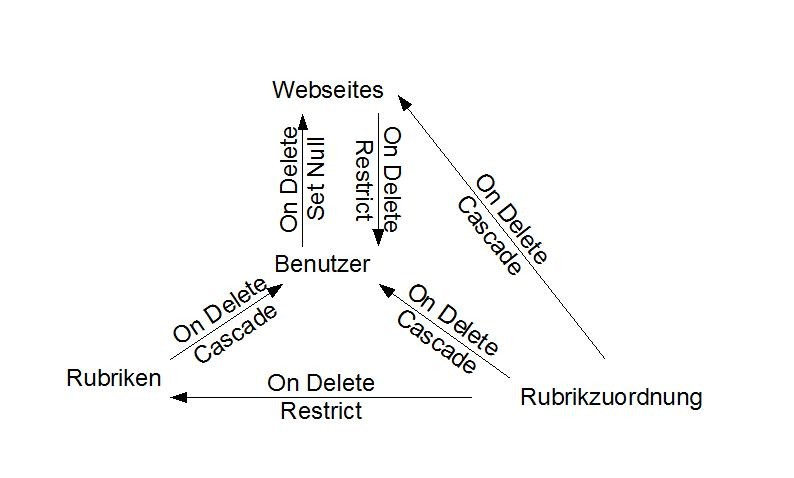
\includegraphics[width=180mm]{gdb1.jpg}
                    \end{figure}

                \item
                    Das Löschen von Benutzer ist reihenfolgenabhängig. Geht man davon aus, dass der Bentuzer keine Webseite eingestellt hat, so kann man entweder die Reihenfolge Benutzer-Rubriken-Rubrikzuordnung wählen, wobei der Löschvorgang abgebrochen wird, aufgrund des Restrict zwischen Rubriken und Rubrikzuordnung oder die Reihenfolge Benutzer-Rubrikzuordnung-Rubriken, die erfolgreich abläuft (Löschen in Benutzer, Löschen in Rubrikzuordnung, Löschen in Rubriken).
                \item
                    Man kann das Restrict zwischen Rubriken und Rubrikzuordnung zu Cascade ändern, oder alle Eingangspfeile von Benutzer zu District ändern. Da der Löschvorgang immer zurückgesetzt wird sobald Benutzer eine Webseite eingestellt hat, ist das Ergebnis in jeder Reihenfolge gleich. 
            \end{enumerate}
        \item
            \begin{enumerate}
                \item 
                    \begin{enumerate}
                        \item 
                            \begin{verbatim}
CREATE VIEW EnterpriseCrew AS
SELECT a.BNr, a.Name, a.Rang 
FROM Besatzungsmitglieder a, Raumschiffe b.
WHERE b.Name  = 'Enterprise'
AND a.Schiff = b.RNr; 
                            \end{verbatim}
                            Sicht nicht änderbar aufgrund des join
                        \item
                            \begin{verbatim}
CREATE VIEW Captains AS
SELECT Name
FROM Besatzungsmitglieder   
WHERE Rang = 'Captain';
                            \end{verbatim}
                        \item 
                            Sicht nicht änderbar da der Primärschlüssel fehlt
                        \item
                            \begin{verbatim}
CREATE VIEW WarpFed AS
SELECT RNr, Fraktion, Baujahr
FROM Raumschiffe
WHERE Geschwindigkeit > 0
AND Fraktion = 'Förderation';
                            \end{verbatim}
                            Sicht änderbar
                    \end{enumerate}
                \item
                    \begin{enumerate}
                        \item 
                            Anweisung durchführbar. Änderungen in der Sicht Förderationsschiffe.
                        \item
                            Anweisung nicht durchführbar, da es die Bedingung Fraktion = 'Förderation' in Förderationsschiffe nicht erfüllt (WITH CASCADED CHECK OPTION)
                        \item
                            Anweisung durchführbar. Änderungen in der Sicht Forschungsschiffe, Förderationsschiffe, GalaxyKlasse
                        \item
                            Anweisung nicht durchführbar, aufgrund der Verletzung der Bedingung Baujahr > 2365 in NebulaKlasse (WITH CASCADED CHECK OPTION)
                        \item
                            Anweisung durchführbar. Änderungen in der Sicht Forschungsschiffe und Förderationsschiffe
                    \end{enumerate}
            \end{enumerate}
    \item
        \begin{enumerate}
            \item[S1:]
                \begin{enumerate}
                    \item A = 305 ; B = 195
                    \item   $r_1(B) \longrightarrow w_2(B)$ \\
                            $r_1(A) \longrightarrow w_2(A)$ \\
                            $w_1(A) \longrightarrow r_2(A)$ \\
                            $w_1(A) \longrightarrow w_2(A)$ \\
                    \item Schedule ist seriell.

                \end{enumerate}
            \item[S2:]
                \begin{enumerate}
                    \item A = 195 ; B = 10
                    \item   $r_2(A) \longrightarrow w_1(A)$ \\
                            $r_1(B) \longrightarrow w_2(B)$ \\
                            $r_1(A) \longrightarrow w_2(A)$ \\
                            $w_2(A) \longrightarrow w_1(A)$ \\
                    \item ⇒ S2 ist nicht serialisierbar. Es gibt keine serielle Abfolge der beiden Transaktionen, die ein identisches
                            Resultat für die Variablen A und B erzielt. Dabei überschreibt Transaktion T1 alle Änderungen an A von T2. (Lost Update)

                \end{enumerate}
            \item[S3:]
                \begin{enumerate}
                    \item A = 300 ; B = 5
                    \item   $r_2(A) \longrightarrow w_1(A)$ \\
                            $w_2(B) \longrightarrow r_1(B)$ \\
                            $w_2(A) \longrightarrow w_1(A)$ \\
                            $w_2(A) \longrightarrow r_1(A)$ \\
                    \item Schedule ist serialisierbar, da alle Abhaengikeiten $T_2$ vor $T_1$ festlegen.
                \end{enumerate}
            \item[S4:]
                \begin{enumerate}
                    \item A = 190 ; B = 5
                    \item   $r_2(A) \longrightarrow w_1(A)$ \\
                            $w_2(B) \longrightarrow r_1(B)$ \\
                            $r_1(A) \longrightarrow w_2(A)$ \\
                            $w_2(A) \longrightarrow w_1(A)$ \\
                    \item S4 ist nicht serialisierbar. Es gibt keine serielle Abfolge der beiden Transaktionen, die ein identisches
                            Resultat für die Variablen A und B erzielt. Dabei überschreibt Transaktion T2 alle Änderungen an T_1. (Lost Update)
                \end{enumerate}
            \item[S5:]
                \begin{enumerate}
                    \item A = 115 ; B = 5
                    \item   $r_2(A) \longrightarrow w_1(A)$ \\
                            $r_1(B) \longrightarrow w_2(B)$ \\
                            $r_1(A) \longrightarrow w_2(A)$ \\
                            $w_1(A) \longrightarrow w_2(A)$ \\
                    \item S5 ist nicht serialisierbar. Es gibt keine serielle Abfolge der beiden Transaktionen, die ein identisches
                            Resultat für die Variablen A und B erzielt. Dabei überschreibt Transaktion T2 alle Änderungen von T1. (Lost Update)
                \end{enumerate}
            \item[S6:] 
                \begin{enumerate}
                    \item A = 305 ; B = 5
                    \item   $r_2(A) \longrightarrow w_1(A)$ \\
                            $w_2(B) \longrightarrow r_1(B)$ \\
                            $w_2(A) \longrightarrow r_1(A)$ \\
                            $w_2(A) \longrightarrow w_1(A)$ \\
                    \item Schedule ist seriell.
                \end{enumerate}
        \end{enumerate}
        \newpage
        $ $
        \item
            \[S = w_1(x) r_2(y) r_3(z) w_3(y) r_2(z) w_3(z) w_1(z) r_2(y) c_3 c_1 c_2 \]
            \renewcommand{\arraystretch}{2}
            \begin{tabular}{|p{1.5cm}|p{1.5cm}|p{1.5cm}|p{1.5cm}|p{0.5cm}|p{0.5cm}|p{0.5cm}|p{2.5cm}|}
                \hline
                Zeitschritt & $T_1$       & $T_2$       & $T_3$       & x     & y     & z     & Bemerkung\\ \hline
                0           &             &             &             & NL    & NL    & NL    & \\ \hline
                1           & lock(x,X)   &             &             & $X_1$ & NL    & NL    & \\ \hline
                2           & write(x)    & lock(y,R)   &             & $X_1$ & $R_2$ & NL    & \\ \hline
                3           &             & read(y)     & lock(z,R)   & $X_1$ & $R_2$ & $R_3$ & \\ \hline
                4           &             &             & read(z)     & $X_1$ & $R_2$ & $R_3$ & \\ \hline
                5           &             &             & lock(y,X)   & $X_1$ & $R_2$ & $R_3$ & $T_3$ wartet auf Freigabe von y\\ \hline
                6           &             & lock(z,R)   &             & $X_1$ & $R_2$ & $R_3$ $R_2$ & \\ \hline
                7           &             & read(z)     & lock(z,X)   & $X_1$ & $R_2$ & $R_3$ $R_2$ & $T_3$ wartet auf Freigabe von z\\ \hline
                8           & lock(z,X)   &             &             & $X_1$ & $R_2$ & $R_3$ $R_2$ & $T_1$ wartet auf Freigabe von z\\ \hline
                9           &             & read(y)     &             & $X_1$ & $R_2$ & $R_3$ $R_2$ & \\ \hline
                10          &             & unlock(y)   &             & $X_1$ & $X_3$ & $R_3$ $R_2$ & $T_3$ wird benachrichtigt\\ \hline
                11          &             & unlock(z)   & write(y)    & $X_1$ & $X_3$ & $X_3$ & $T_3$ wird benachrichtigt\\ \hline
                12          &             &             & write(z)    & $X_1$ & $X_3$ & $X_3$ & \\ \hline
                13          &             &             & unlock(y)   & $X_1$ & NL    & $X_3$ & \\ \hline
                14          &             &             & unlock(z)   & $X_1$ & NL    & $X_1$ & $T_1$ wird benachrichtigt \\ \hline
                15          & write(z)    &             & commit      & $X_1$ & NL    & $X_1$ & \\ \hline
                16          & unlock(x)   &             &             & NL    & NL    & $X_1$ & \\ \hline
                17          & unlock(z)   &             &             & NL    & NL    & NL    & \\ \hline
                18          & commit      &             &             &       &       &       & \\ \hline
                19          &             & commit      &             &       &       &       & \\ \hline
        \end{tabular}
    \end{enumerate}
\end{document}
